\chapter{Installation}
\label{chapter:Installation}

\index{Installation}

Ce chapitre d\'{e}crit les proc\'{e}dures pour installer l'OTB sur votre syst\`{e}me.
Vous devez avant tout compiler l'OTB pour pouvoir l'utiliser et cr\'{e}er vos propres applications.


L'OTB s'appuie sur un ensemble de biblioth\`{e}ques externes de type libre (licence GNU/GPL, etc...) qu'il est n\'{e}cessaire de disposer sur votre syst\`{e}me.
Ces biblioth\`{e}ques sont les suivantes :
\begin{itemize}
\item ITK\footnote{http://www.itk.org} (\emph{Insight Toolkit}) utilis\'{e}e comme base de d\'{e}veloppement de l'OTB, pour tous les traitements de filtrage, recalage, segmentation, etc...
\item VTK\footnote{http://www.vtk.org} (\emph{Visualization ToolKit}) utilis\'{e}e pour la visualisation des donn\'{e}es
\item FLTK\footnote{http://www.fltk.org}(\emph{Fast Light Toolkit}) utilis\'{e}e pour la ralisation d'IHM graphiques
\item GDAL\footnote{http://www.remotesensing.org/gdal/} (\emph{Geospatial Data Abstraction Library}) utilis\'{e}e pour toutes les fonctionnailt\'{e}s de lecture et d'\'{e}criture des images de t\'{e}l\'{e}d\'{e}tection
\item CAI (\emph{Couche d'Acc\`{e}s Images}) utilis\'{e}e pour la lecture et l'\'{e}criture des images non support\'{e}es par GDAL, en particulier pour les formats d'images SPOT.
\item GSL\footnote{http://www.gnu.org/software/gsl/} (\emph{GNU Scientific Library}) utilis\'{e}e pour toutes les fonctionnalit\'{e}s math\'{e}matiques 
tr\`{e}s sp\'{e}cifiques et non fournies par ITK
\item SVM\footnote{http://www.csie.ntu.edu.tw/~cjlin/libsvm/} (\emph{Support Vector Machines}) utilis\'{e}e pour la mise en oeuvre des outils d'apprentissage par \emph{SVM}
\end{itemize}

Elles peuvent \^{e}tre t\'{e}l\'{e}charg\'{e}es sur les sites r\'{e}f\'{e}renc\'{e}s ci-dessus par les liens.



L'OTB a \'{e}t\'{e} d\'{e}velopp\'{e}e et test\'{e}e sur plusieurs types de plate-formes op\'{e}rationnelles telles que \emph{Microsoft Windows}, 
\emph{Linux} (machine compatible \emph{Intel}), \emph{Solaris}, and \emph{Cygwin}.
Il est ainsi possible d'utiliser les compilateurs suivants :
\begin{itemize}
\item Visual Studio 6
\item GCC 2.95.x, 2.96, 3.x
\end{itemize}

\section{Configurer l'OTB}
\label{sec:ConfigurerOTB}

\index{Configuration}
 
L'environnement de l'OTB est mis en place via l'outil CMake\footnote{http://www.cmake.org}, 
permettant ainsi de g\'{e}rer les proc\'{e}dures de compilation, g\'{e}n\'{e}ration et d'installation de syst\`{e}mes, et ce quelque sois la plate forme cible.

CMake permet de g\'{e}n\'{e}rer les \emph{Makefiles} pour les syt\`{e}mes UNIX, Cygwin et les \emph{Workspaces} pour l'environnement Visual Studio de Microsoft.

CMake utilise les informations contenues dans les fichiers nomm\'{e}es \code{CMakeLists.txt} pr\'{e}sents dans chaque r\'{e}pertoire de l'OTB.
L'utilisateur d\'{e}crit dans ces fichiers l'information n\'{e}cessaire pour que CMake puisse configurer son syst\`{e}me (recherche de librairies externes d\'{e}j\`{a} install\'{e}es sur votre syst\`{e}me, etc...)

\subsection{Pr\'{e}parer CMake}
\label{sec:CMakeforOTB}
 
\index{CMake}
\index{CMake!downloading}

CMake peut \^{e}tre t\'{e}l\'{e}charg\'{e} depuis le site
\begin{center} 
  \url{http://www.cmake.org}
\end{center}

La version 2.0 de CMake est la version minimale requise pour configurer l'OTB.
Vous pouvez t\'{e}l\'{e}charger les versions "binaires" de la plupart des plates-formes comme Windows, Solaris, IRIX, HP, Mac et Linux.

Il est aussi possible de t\'{e}l\'{e}charger les sources de CMake sur votre syst\`{e}me et de re-g\'{e}n\'{e}rer l'application. 
Les instructions sont disponibles sur le site Internet de CMake \url{http://www.cmake.org}.


Pour ex\'{e}cuter CMake, il est n\'{e}cessaire de d\'{e}finir :
le r\'{e}pertoire des sources (OTB\_SOURCE\_DIR), 
et le r\'{e}pertoire o\`{u} sont produits les fichiers binaires (OTB\_BINARY\_DIR). 

Il est r\'{e}command\'{e} d'installer et de compiler les fichiers binaires dans un r\'{e}pertoire autre que le r\'{e}pertoire des sources de l'OTB. 
Par exemple :

\small
\begin{verbatim}
mkdir OTB-bin
cd OTB-bin
ccmake ../OTB
\end{verbatim}
\normalsize

Sous Windows, l'interface GUI de CMake est utilis\'{e}e pour d\'{e}finir et construire les r\'{e}pertoires (Figure \ref{fig:CMakeGUI}).

CMake se lance en mode int\'{e}ractif, o\`{u} il est possible de configurer certains param\`{e}tres et valider des options.
L'\'{e}tape de configuration permet alors de g\'{e}n\'{e}rer les fichiers de configuration.


\subsection{Configurer l'OTB}
\label{sec:ConfiguringITKwithVTK}
  
\index{Configuration!with VTK}

La Figure \ref{fig:CMakeGUI} montre l'interface CMake pour UNIX et Windows.

\begin{figure}[ht]
\centering 
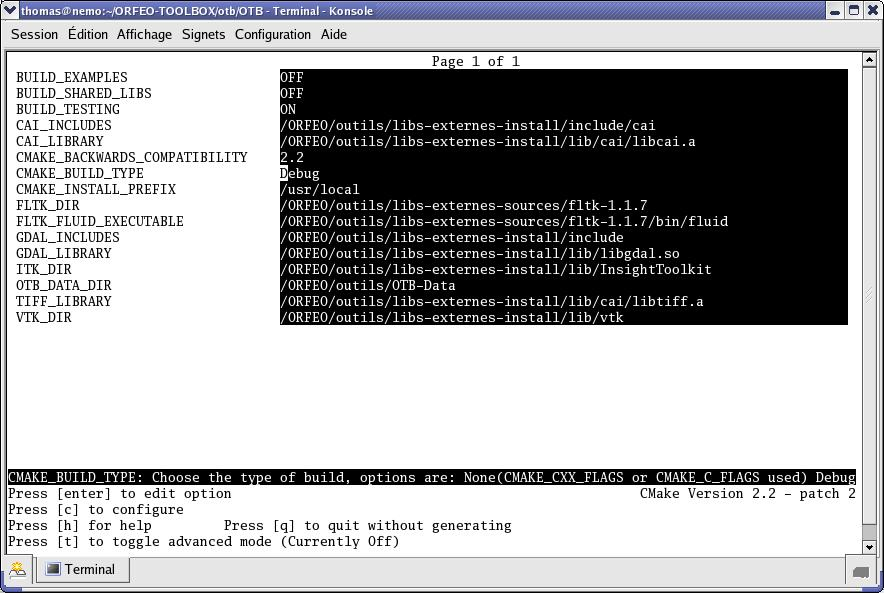
\includegraphics[width=0.8\textwidth]{ccmakeScreenShot.eps}
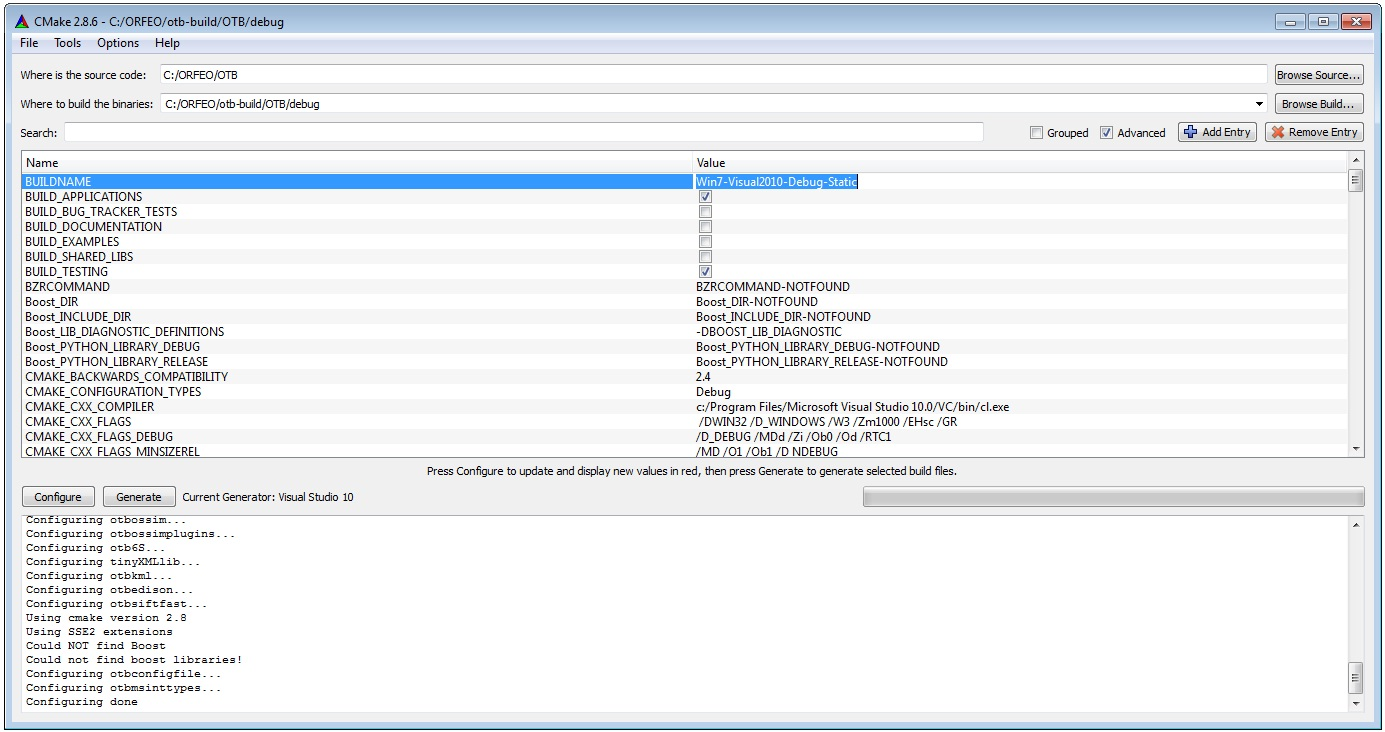
\includegraphics[width=0.8\textwidth]{CMakeSetupScreenShot.eps}
\itkcaption[Interface utilisateur de CMake]{Interface CMake. En Haut) \texttt{ccmake}, interface sous UNIX. En Bas) \texttt{CMakeSetup}, 
la version MS-Windows pour les MFC.}
\label{fig:CMakeGUI}
\end{figure}

Il est possible de choisir si l'on souhaite compiler les exemples (\code{OTB/Examples}) et les tests (\code{OTB/Testing}).
Ceci est possible en positionnant les variables \code{BUILD\_EXAMPLES=OFF} et \code{BUILD\_TESTING=OFF}.

Ces exemples peuvent \^{e}tre utilis\'{e}s pour se familiariser avec l'OTB. Les tests sont constitu\'{e}s 
d'un ensemble de petits programmes permettant de valider l'OTB.
De plus, le composant \code{OTB-Applications} montrent des applications plus \'{e}volu\'{e}es, utilisant notamment des IHM 
graphiques et de la visualisation.


\section{D\'{e}marrer avec l'OTB}
\label{sec:GettingStartedWithOTB}
 
\subsection{Hello World !}
\label{sec:HelloWorldOTB}

\index{Hello World}

Cet exemple permet de montrer comment cr\'{e}er un petit programme, qui utilise la biblioth\`{e}que OTB 
(cet exemple se trouve dans le r\'{e}pertoire \code{OTB/Examples/Installation}).
Le fichier \code{CMakeLists.txt} contient les lignes suivantes :

\small
\begin{verbatim}
PROJECT(HelloWorld)

FIND_PACKAGE(OTB)
IF(OTB_FOUND)
  INCLUDE(${OTB_USE_FILE})
ELSE(OTB_FOUND)
  MESSAGE(FATAL_ERROR
          "OTB non trouvee. Positionner la variable OTB_DIR.")
ENDIF(OTB_FOUND)

ADD_EXECUTABLE(HelloWorld HelloWorld.cxx )

TARGET_LINK_LIBRARIES(HelloWorld OTBCommon)
\end{verbatim}
\normalsize

La premi\`{e}re ligne d\'{e}finie le nom du projet pour l'environnement Visual Studio (n'a aucun effet sous UNIX).
 La seconde ligne pr\'{e}cise que la biblioth\`{e}que OTB est n\'{e}cessaire pour compiler ce programme. 
Si elle n'est pas trouv\'{e}e, un message d'erreur est \'{e}mis.
La ligne \code{ADD\_EXECUTABLE} permet de d\'{e}finir le programme que l'on cr\'{e}\'{e}e 
(le premier argument est le nom de l'ex\'{e}cutable, les suivants le(s) fichier(s) source(s) associ\'{e}(s) \`{a} cet ex\'{e}cutable)
La ligne \code{TARGET\_LINK\_LIBRARIES} pr\'{e}cise quelles biblioth\`{e}ques sont n\'{e}cessaires pour g\'{e}n\'{e}rer cet ex\'{e}cutable.

\input HelloWorld.tex

Vous avez maintenant install\'{e} et compil\'{e} avec succ\`{e}s la biblioth\`{e}que OTB, et vous avez cr\'{e}\'{e} un programme simple se \emph{linkant} avec cette biblioth\`{e}que.
Si vous avez des difficult\'{e}s, vous pouvez prendre contact avec les auteurs de ce document.

